\subsection{Ordnerstruktur}

\subsubsection{Übersicht der obersten Ordnerstruktur}
Der Quelltextdateien, welche die Anwendungen beschreibt, sind innerhalb des Ordner \textit{src} organisiert. 
Die obersten Ordnerebene des \textit{src}-Ordner spiegelt die Architektur der Anwendung auf höchster Ebene wider. 
Mit Hilfe des Analysewerkzeug \textit{Dependency cruiser} wurde Abbildung \ref{fig:obersteOrdnerebene}  erstellt, welche eine Übersicht der obersten Ordnerebene gibt, sowie einen Überblick der Zugriffe zwischen den Ordnern. Wird innerhalb eines Ordners Quelltext aus einem benachbarten Ordner importiert, wird dies durch eine Pfeilspitze am benachbarten Ordner gekennzeichnet. 

\begin{figure}[H]
	\centering
	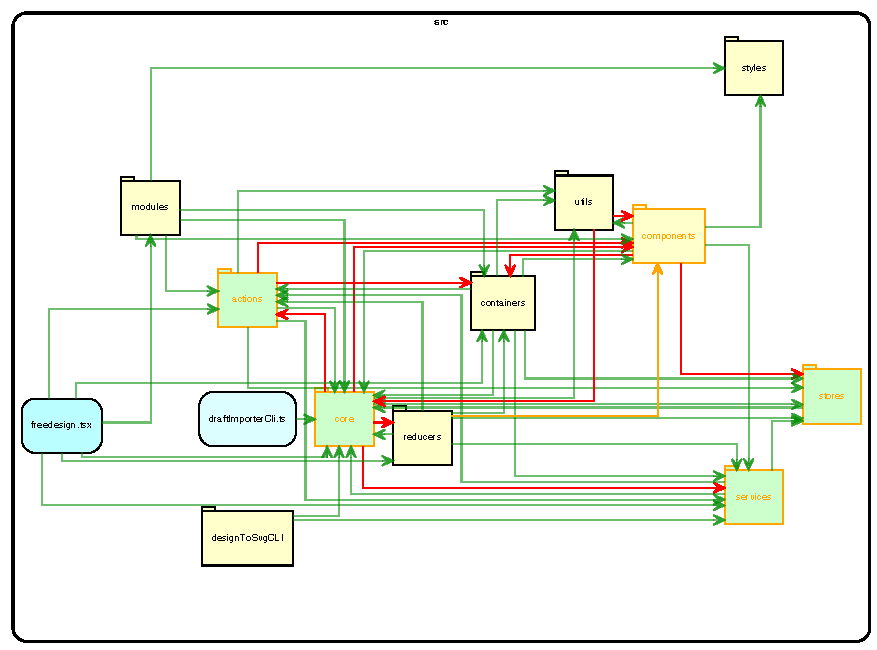
\includegraphics{diagrams/Ist-Architektur/high-level-graph.pdf}
	\caption{Eine Übersicht der obersten Ordnerebene, sowie ein Überblick der Zugriffe zwischen den Ordern.}
	\label{fig:obersteOrdnerebene}
\end{figure}


\paragraph{freedesign.tsx \& draftImporterCli.ts}
Die Datei \textit{freedesign.tsx} ist die Startdatei der FreeDesign-Anwendung, über die das Programm betreten wird. Für das Kommandozeilen-Programm \textit{Draft-Importer} ist die Datei \textit{draftImporterCli.ts} als Startdatei vorgesehen. 

\subsubsection{Der \textit{modules}-Ordner}
Für die Anwendung sollten mehrerer Einstieg-Möglichkeit geschaffen werden. 

\subsubsection{Der \textit{core}-Ordner}
Der \textit{core}-Ordner enthält Domain-Logik sowie grundlegende Funktionalitäten und Datenstrukturen der Anwendung, die nicht direkt mit ReactJS und Redux im Zusammenhang stehen. 
Die Hierarchie innerhalb des Ordners ist sehr flach gehalten.  
Es soll der \textit{core}-Ordner lediglich von Anwendung genutzt werden. Er selber darf nicht an sie gebunden sein.  Daher sollten keine Zugriffe auf Quelltext innerhalb der umgebenden Ordner stattfinden. 


\begin{figure}[H]
	\centering
	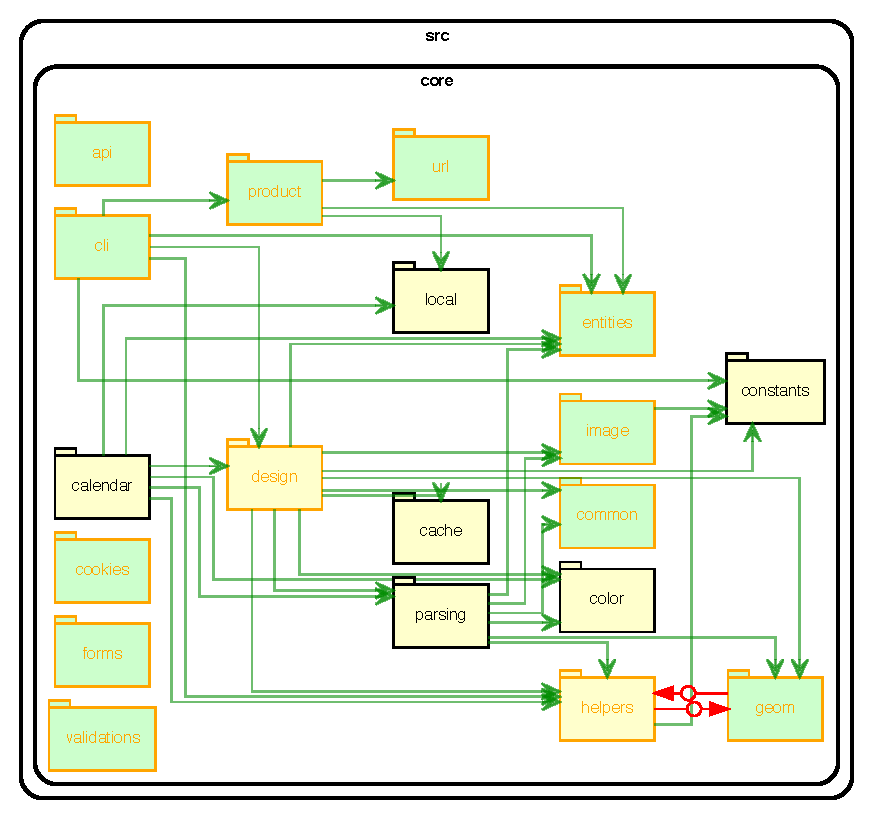
\includegraphics{diagrams/Ist-Architektur/core-graph.pdf}
	\caption{Übersicht  }
	\label{fig:coreGraph}
\end{figure}

\subsubsection{Der \textit{services}-Ordner}
Im Ordner \textit{services} sind größtenteils die Aufruf der API definiert, sowie zugehörige Datenstruktur. 

\subsubsection{Der \textit{utils}-Ordner}
Der Ordner \textit{utils} ist ein sehr kleines Ordner mit zwei Komponenten, die direkt mit der Browser-API kommunizieren und sich nur innerhalb des Browser aufrufen lassen. 

\subsubsection{Der \textit{components}-Ordner}

\subsubsection{Die Ordner \textit{stores}, \textit{actions} \& \textit{reducers}}
Im Ordner \textit{store} ist die Struktur des \textit{Redux-State} abgelegt.  Unter \textit{actions} und \textit{reducers}  sind die \textit{Redux-Actions}, sowie die \textit{Redux-Reducer}. Die Action-

%TODO alle haben eine ebene

\subsubsection{Der \textit{containers}-Ordner}

\subsubsection{Der \textit{styles}-Ordner}

\subsubsection{Der \textit{designToSvgCLI}-Ordner}

